\documentclass[12pt, a4]{report}
\usepackage[utf8]{inputenc}
\usepackage[margin=0.8in]{geometry}
\def\thesection{\arabic{section}}
\setcounter{tocdepth}{4}

%
% ─── IMPORTS ────────────────────────────────────────────────────────────────────
%
\usepackage{graphicx}
\graphicspath{ {images/} }
\usepackage{listings}
\usepackage{verbatim}
\usepackage{color}
\usepackage{csquotes}
\usepackage{opensans}

%
% ─── TABLE CONFIGURATIONS ───────────────────────────────────────────────────────
%
\setlength{\arrayrulewidth}{0.5mm}
\setlength{\tabcolsep}{10pt}
\renewcommand{\arraystretch}{1.5}

%
% ─── STYLING AND CONFIGURATION FOR CODE LISTING ─────────────────────────────────
%
\definecolor{codegreen}{rgb}{0,0.6,0}
\definecolor{codegray}{rgb}{0.5,0.5,0.5}
\definecolor{codepurple}{rgb}{0.58,0,0.82}
\definecolor{backcolour}{rgb}{0.95,0.5,0.92}
\definecolor{bittersweet}{rgb}{1.0, 0.44, 0.37}
\definecolor{cosmiclatte}{rgb}{0.93, 0.93, 0.93}
\definecolor{eggshell}{rgb}{0.94, 0.94, 0.9}
\definecolor{fandango}{rgb}{0.71, 0.2, 0.54}
% \definecolor{fawn}{rgb}{0.9, 0.67, 0.44}
\definecolor{fawn}{rgb}{0.89, 0.45, 0.36}
\lstdefinestyle{mystyle}{
	backgroundcolor=\color{cosmiclatte},   
	commentstyle=\color{codegreen},
	keywordstyle=\color{fandango}\small,
	numberstyle=\tiny\color{codegray},
	stringstyle=\color{codepurple},
	basicstyle=\ttfamily\footnotesize,
	breakatwhitespace=false,        
	breaklines=true,               
	captionpos=b,                    
	keepspaces=true,  
	numbers=left,                    
	numbersep=5pt,                  
	showspaces=false,                
	showstringspaces=false,
	showtabs=false,                  
	tabsize=2
}
\lstset{style=mystyle}

%
% ─── COVERPAGE ──────────────────────────────────────────────────────────────────
%
\title{2810, Principles of Software Engineering Milestone 02}
\author{Zaymon Foulds-Cook, s5017391}%\thanks{}}
\date{\today}
\begin{document}
\begin{titlepage}
	\maketitle
\end{titlepage}

\tableofcontents
\pagebreak

%
% ─── START OF REPORT ────────────────────────────────────────────────────────────
%
\section{Software Technologies Assignment 1}
\subsection{Requirements}
\par Throughout this software project various software requirements have been identified. The following list itemizes each requirement and discusses the current completion status of each item.
\begin{itemize}
	% \par \textcolor{codegreen}{Implemented - ongoing \textbar{} } 
	\item Create system models for structure and behaviour of software products.
	\par \textcolor{codegreen}{Implemented - ongoing \textbar{} } Various models have been created of the software system which allow team members to make architectural decisions as well as gain high level overviews of the software system.
	
	\item Select appropriate software architecture
	\par \textcolor{codegreen}{Implemented - ongoing \textbar{} } The model view controller architecture was chosen for this project and has been fully implemented. The software systems adheres strictly to MVC for interactions, data flow and structure. 

	\item Make use of appropriate design patterns
	\par \textcolor{codegreen}{Implemented - ongoing \textbar{} } Various software design patterns have been used throughout the project such as the `façade pattern' and the `model view controller pattern'. More patterns such as singleton will be implemented in the final software system.

	\item Create user interface software using event driven or call-back based designs
	\par \textcolor{codegreen}{Implemented - ongoing \textbar{} } The software system has a user interface which is driven by call-back based interactions with the game board.

	\item Create a model `state' representation of the minesweeper game which is generalizable to many different configurations of the minesweeper such as `hex-mines' and `colour-mode'
	\par \textcolor{fawn}{Implemented - to be extended \textbar{} } The board model in the program is generalizable to many different configurations but the hex and colour mode specific implementation is not completed. However, the board state is very versatile and extensible and further implementations should be easily introduced.

	\item Create a controller object which mutates the game state
	\par \textcolor{codegreen}{Implemented - Complete \textbar{} } The game controller is full completed.

	\item Create a main menu which allows the user to select the game mode and difficulty
	\par \textcolor{fawn}{Implemented - to be extended \textbar{} } The main menu currently starts a game correctly and passes parameters back to the parent object on destruction. The main menus functionality will be completed soon when the final game modes are implemented.

	\item Create reusable GUI components
	\par \textcolor{codegreen}{Implemented - ongoing \textbar{} } The main menu, view, and menu bar objects all extend Frame and can be reused.

	\item Create an extensible view object which can adapt to multiple different implementations of the minesweeper game
	\par \textcolor{fawn}{Implemented - to be extended \textbar{} } The current view object uses the model and controller to draw images to the canvas. The view is easily extended and implementing the remaining game modes is straightforward. The current view works for the square implementation of the minesweeper game.
\end{itemize}

\subsection{Product Use Cases}
\par 

\subsection{Summary of Software Architecture}
\par Software architecture is a set of guidelines principles models and processes. The software architecture being used in the minesweeper software system is based around the model view controller software pattern. The Minesweeper software system has been written and implemented purely in python and uses the tkinter user interface library which comes bundled with a typical install of python. No integrated development environments have been used throughout the development process as the developer has opted to simply use the Visual Studio code text editor. 
\newline
\par The modules and components of the Minesweeper software system have been structured in a manner to: reduce coupling, increase cohesion, increase modularity and to enforce a clear separation of concerns between logically related collections of code. The main class of the game MineSweeper is the overarching class and contains objects of the model view and controller classes. The model class represents the internal game-state and does not have a reference to any other class. The controller class is responsible for mutating data in the model by calling the models mutator functions. The controller class does not have a reference to the view. Review class has a reference to both of the controller and the model. The view gets the current state of the model and displays it to the user via a graphical representation. When handling and call back event the view interacts with the model through the controller and the controller acts like a thin proxy or API for the model. This separation between view model and controller allows the internal representation to be changed without impacting interactions between the view and the model. 
\newline
\par The software architecture used in this project enforces modularity by design and allows for a clear separation of concerns. It is highly feasible that the software architecture will remain the same until the project completion as the software architecture allows for highly extendable code and changes can be easily made without cascading changes being needed throughout the project source.

\subsection{Summary of Design}
\par Since milestone 1 it has become apparent that some design goals needed to be created in order to improve the overall effectiveness of the software system in terms of code quality, maintainability and structure. The design goals chosen for the project are: minimising coupling, maximising cohesion, optimising response time, facilitating maintenance and increasing modularity.
\subsubsection{Minimising Coupling}
The original software system for the Milestone 1 submission demonstrated had high levels of coupling. The software system consisted of one file and different components within the system depended on one another. The view and model state representation were highly coupled as the view contain data we should have been reserved for the state. By following the model view controller software pattern I was able to reduce code interdependence and provide a clearer separation of concerns.


\subsubsection{Maximising Cohesion}
As the Milestone one submission had a high level of coupling it also had a low level of cohesion. As the software system was one module, the level of cohesion was very low as functions and pieces of code with very different purpose and functionality existed in the same module. An effort to increase cohesion has been made by dividing the original program into multiple different modules of similar functionality. An example of this would be the interdependence of the view and the model. Before the program restructure, code that modified the internal state of the board was bundled together with code that create the graphical user interface and the view. After the program restructure separation of concerns has been maximised by only allowing logically related functions and code to exist in the same module.

\subsubsection{Optimising Response Time}
An effort has been made to improve the response time of the minesweeper application. A big positive impact was only re-rendering the game view after a complete change in the game-state. An issue that affected earlier versions of the Minesweeper game was the cascading reveal being progressively rendered across the view as it relied on button components. Since switching the game to a canvas based render system the response time has been vastly improved to the point where rendering stat changes is imperceptible to the user.

\subsubsection{Facilitating Maintenance}
Since the start of the project the maintainability of the software system has increased dramatically. Increases and readability and decreases and coupling along with effective commenting and increases in understandability. Functions and variable names have been refactored to be more explicit in conveying the purpose and functionality of the code. By abstracting common tasks into functions there is reduced redundancy within the source code. Another increase to the maintainability of the software system is following proper naming conventions for variables and classes.

\subsubsection{Increasing Modularity}
The increase in modularity can be directly attributed to restructuring the software system to follow the model view controller software pattern. During the restructure common code and functions we're grouped together in various models based on similarities in functionality. An example of this would be the view only containing functions related to rendering the graphical user interface and handling events. Functions such as draw\_tile() and populate\_buttons() are logically related and belong in the same class. It is evident from the object model that each module in the software system contains function specific to that module. The increase in modularity strongly reinforces a good separation of concerns as each core module does not depend on the existence and state of other modules. An increase in modularity is desirable as it allows modules to be replaced or implementations to be changed without cascading changes being required throughout the software system.

\subsection{Summary of Design, Diagrams}
\begin{figure}[!h]
	\centering
	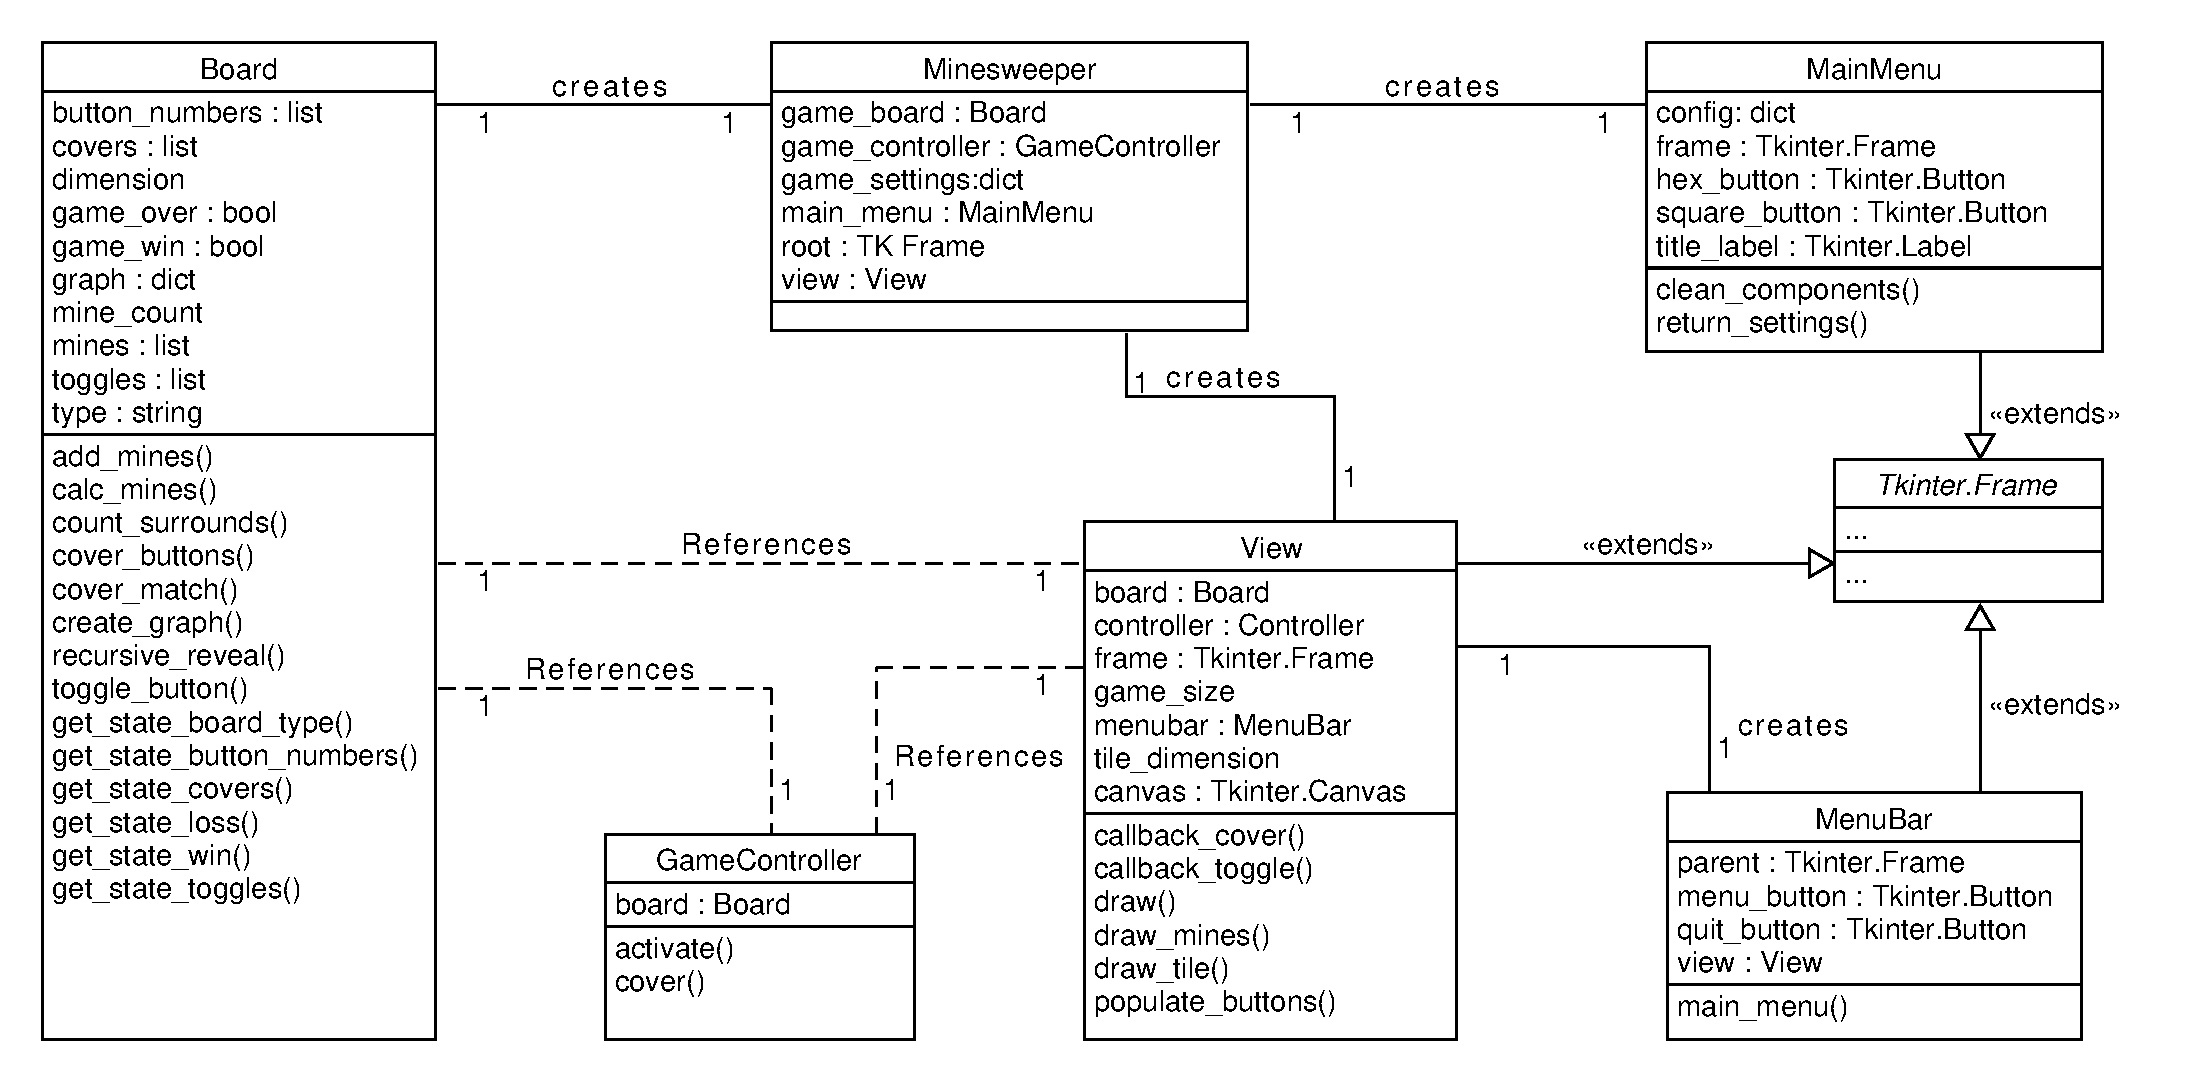
\includegraphics[scale=0.5]{ClassDiagram}
	\caption{UML diagram for the Python implementation of Ladder-gram}
\end{figure}
\par 

\begin{figure}[!h]
	\centering
	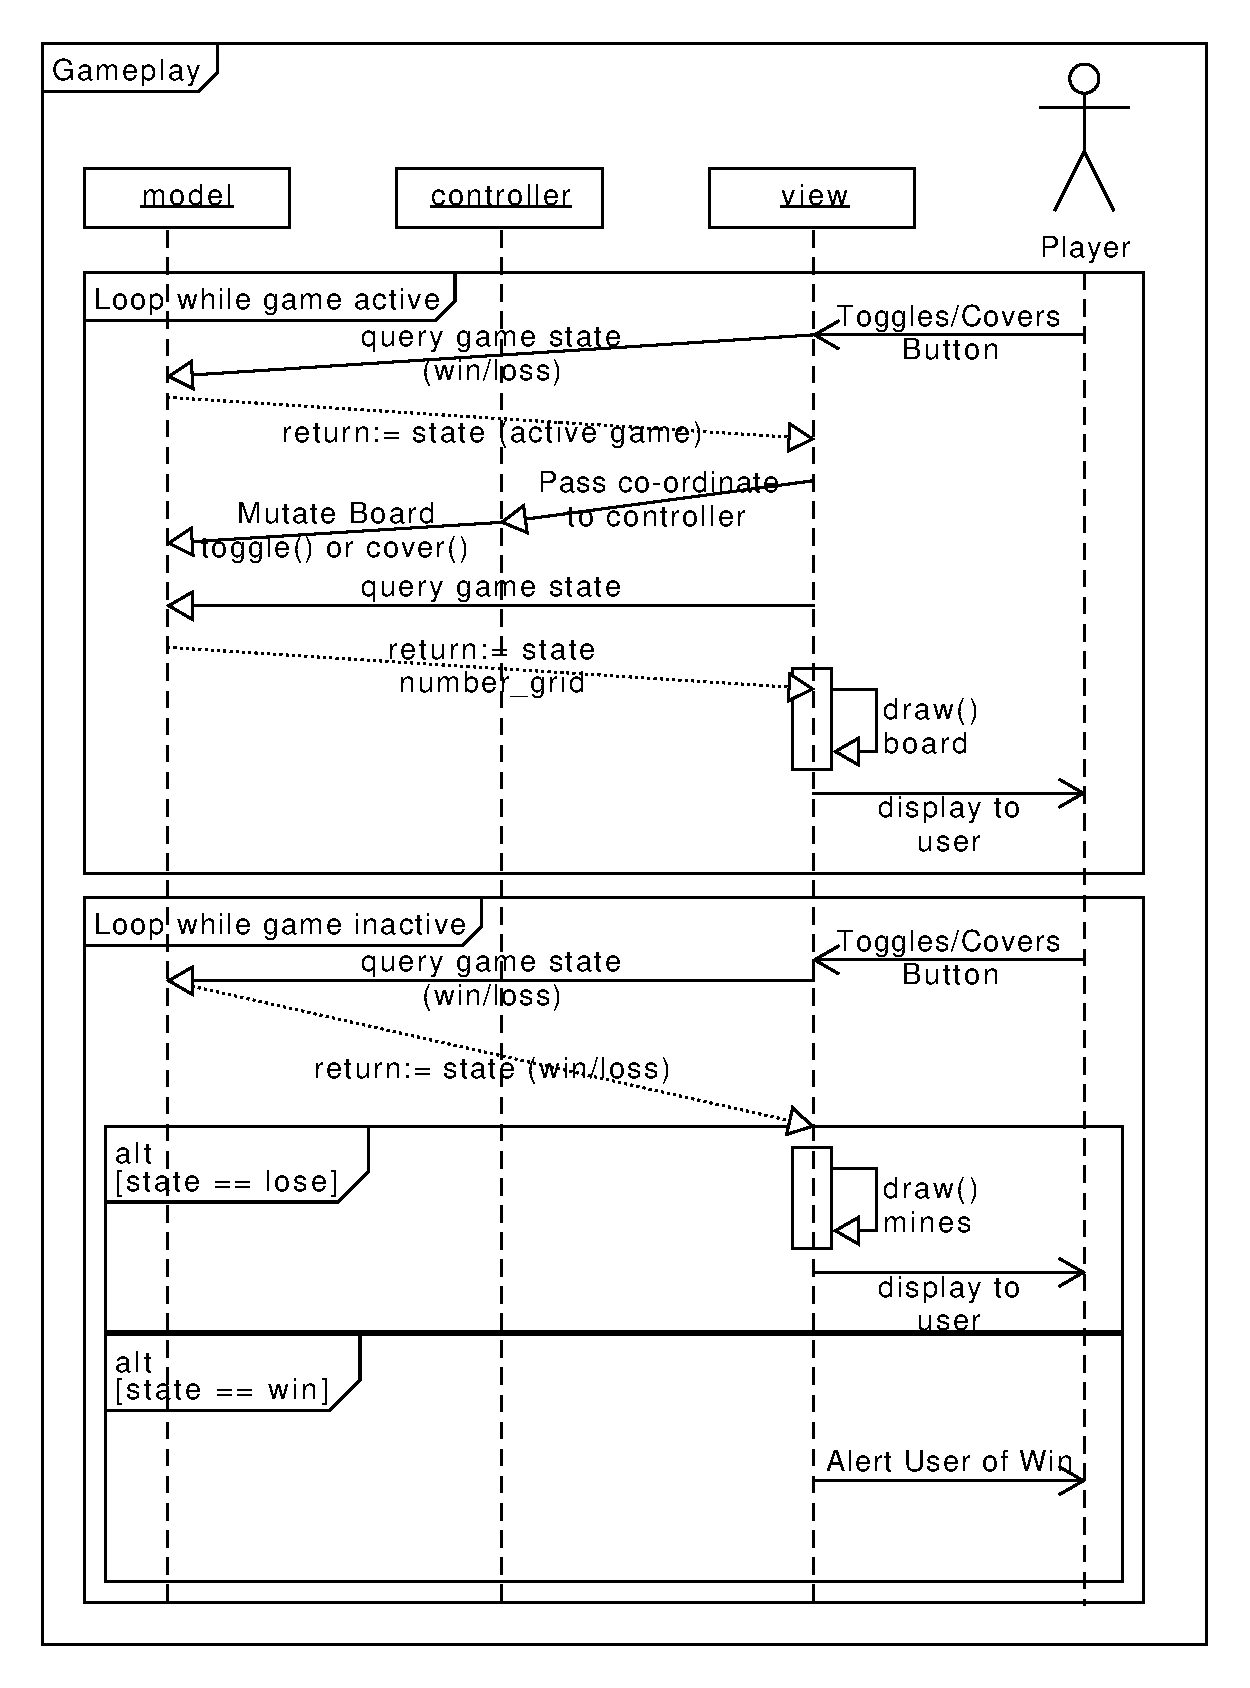
\includegraphics[scale=0.7]{SequenceDiagram}
	\caption{UML diagram for the Python implementation of Ladder-gram}
\end{figure}
\begin{figure}[!h]
	\centering
	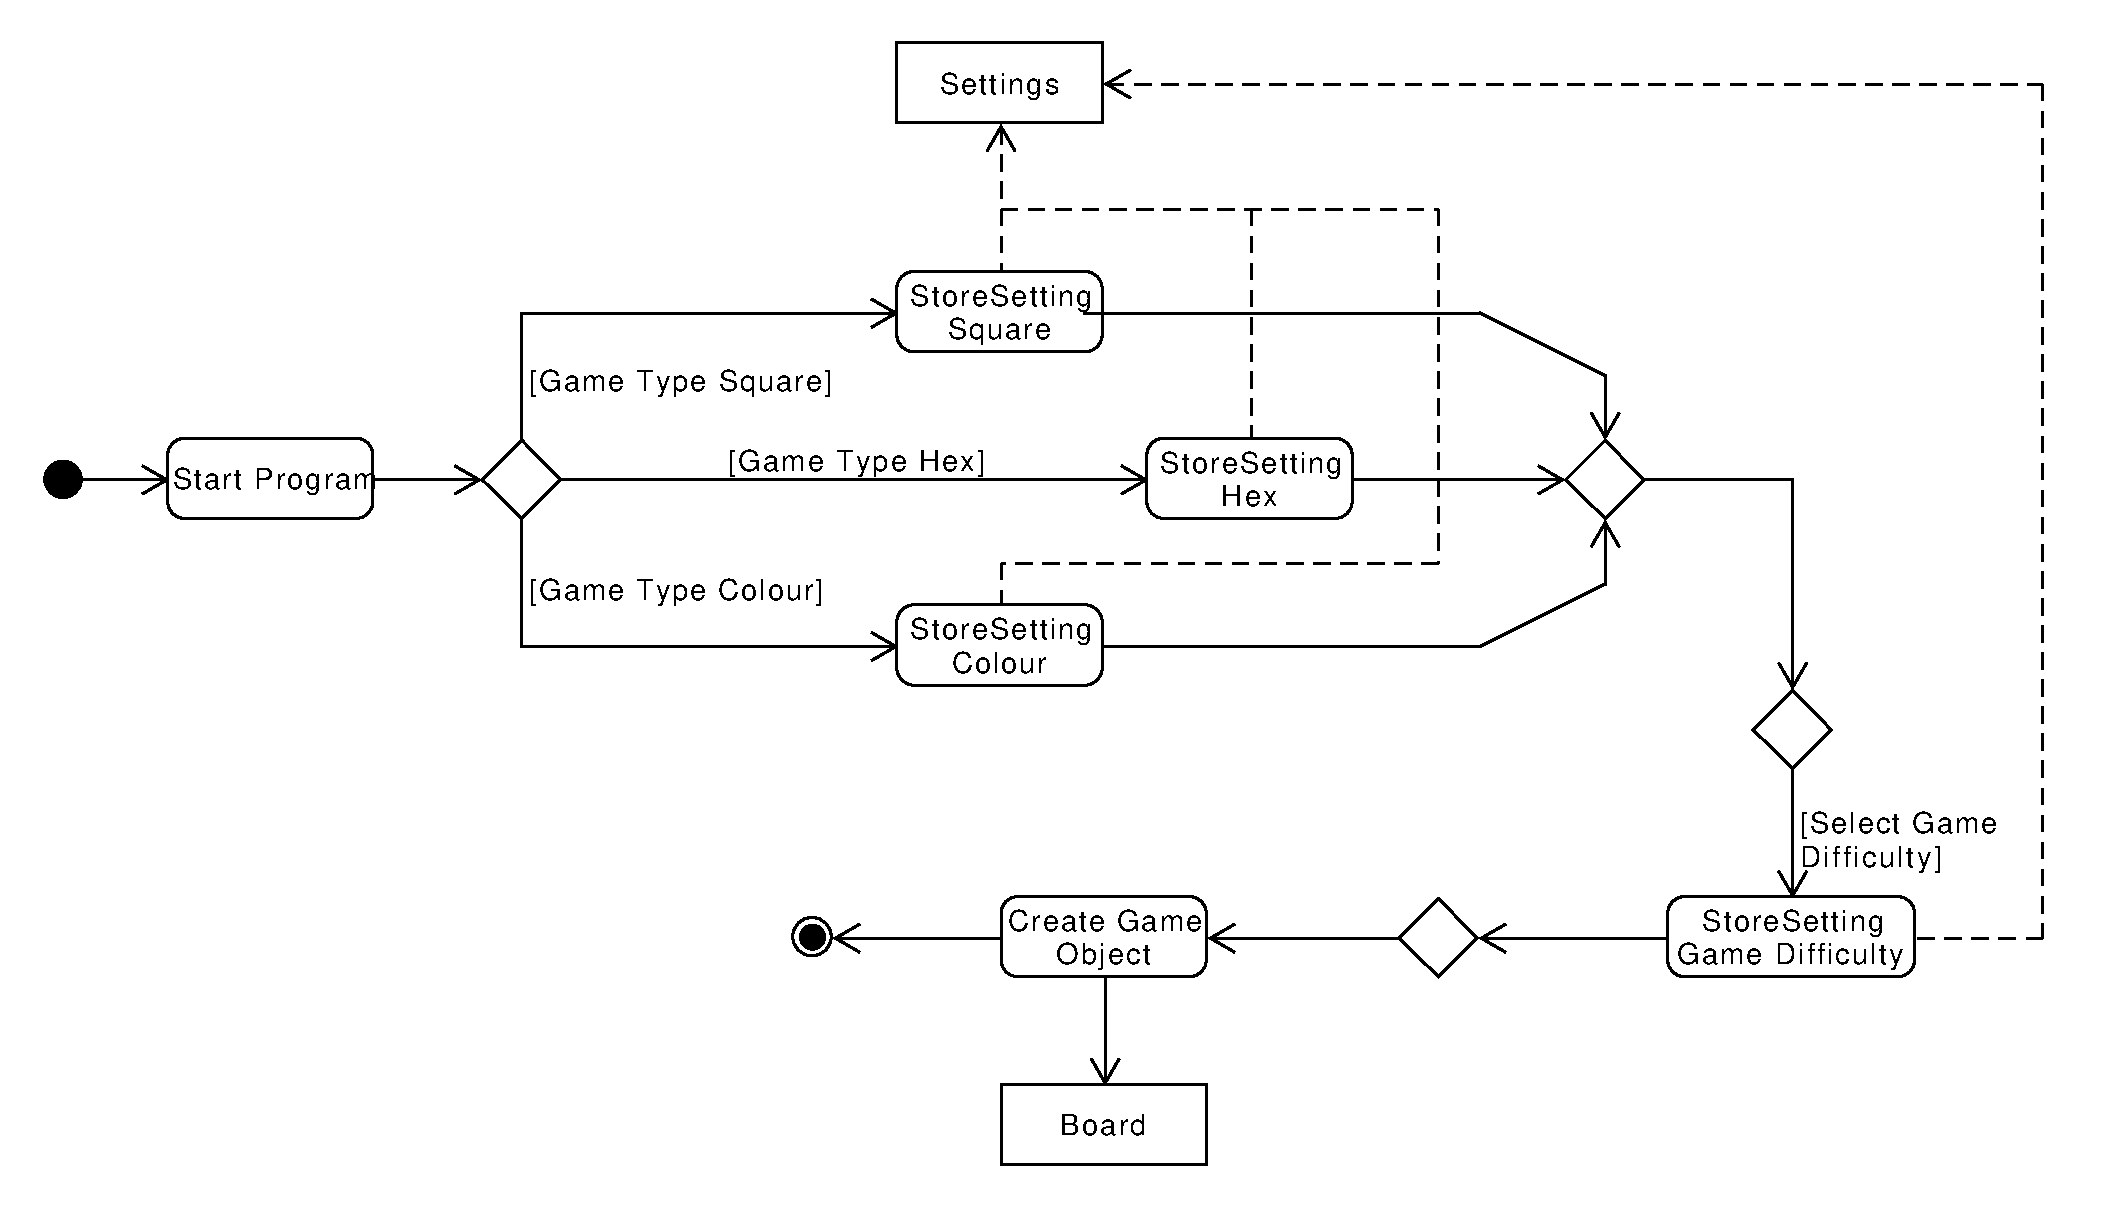
\includegraphics[scale=0.5]{ActivityDiagram}
	\caption{UML diagram for the Python implementation of Ladder-gram}
\end{figure}
\begin{figure}[!h]
	\centering
	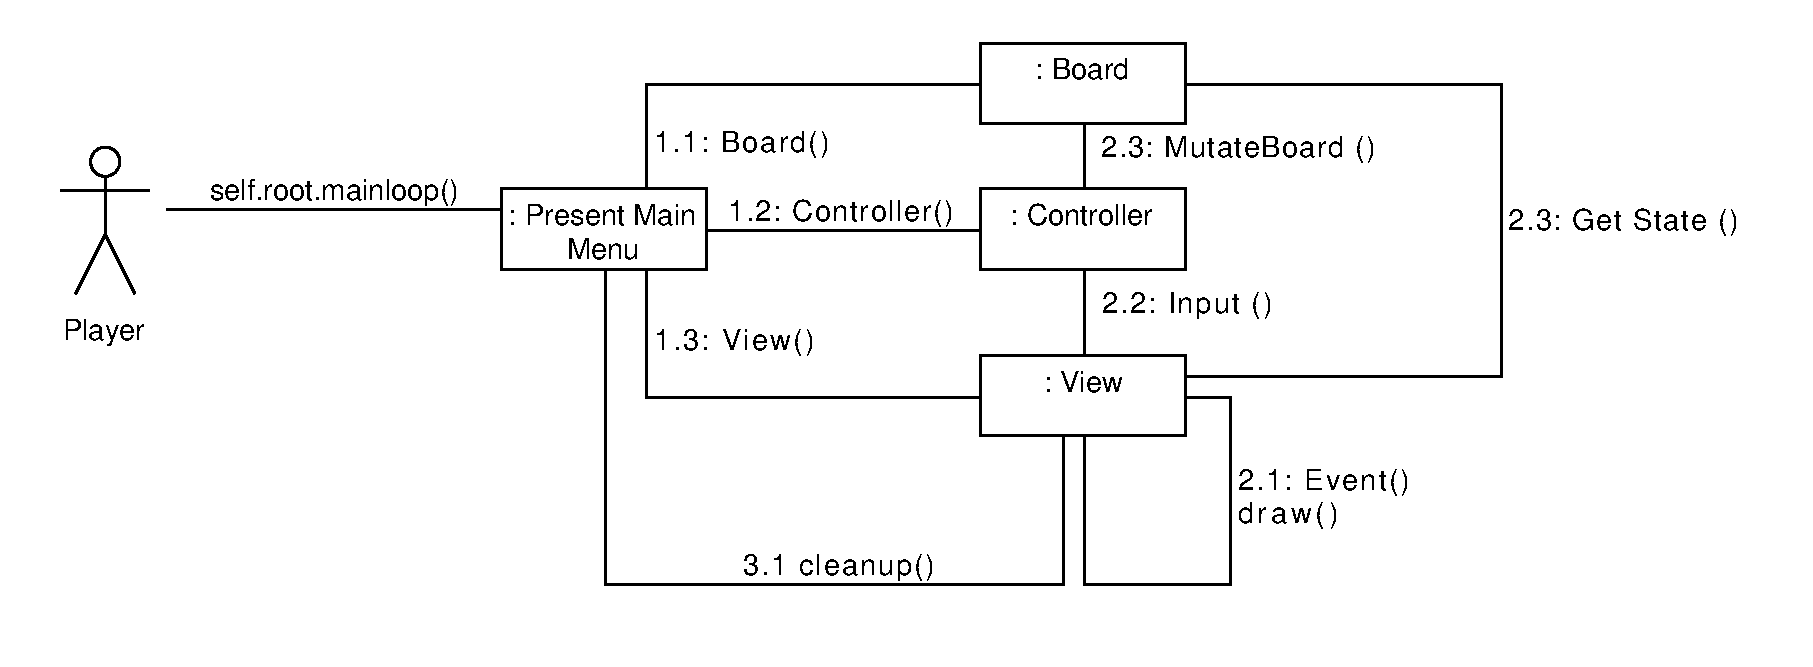
\includegraphics[scale=0.6]{CollaborationDiagram}
	\caption{UML diagram for the Python implementation of Ladder-gram}
\end{figure}


\subsection{Discussion of Sophistication Regarding Persistent Data Management, Access Control and User Interface}
\subsubsection{Persistent Data Management}
In the Minesweeper software system there is no persistent data stored in between games at this point in the game's development. Depending on your timeline there may be a need for a persistent data service in order to store user high scores. High scores are not a critical functional requirement and of the implementation of this data store is dependent on the workflow and time management of the developer.

\subsubsection{Access Control}
As there are no access restricted sections of the game and the software system currently only runs locally on a user's computer access control has not been a significant feature of the Minesweeper program. However, the security of the application is important as tampering could potentially put the user at risk. As the application does not run with root privileges and the user will be provided with a compiled binary, a security breach of the user's operating system or escalation of privileges is unlikely. As the software system is not exposed to the network remote security concerns do not need to be addressed within the scope of this product's development.

\subsubsection{User Interface}
The user interface for the software system of Minesweeper is quite sophisticated. It is built on top of the python tkinter library to create frames and components. The various sections of the user interface used in this application have been split into modules which subclass the tkinter frame object. This allows different UI components to be laid out in various configurations and increases maintainability as each component is limited in scope and functionality. This also enhances the re-usability of the code as models can be re-purposed in different situations. The user interface draws the tiles by rendering images onto a tkinter canvas object. This allows the game board to be very responsive and will make it easier to implement different views based on different configurations of the game by only changing a small subset of the code.

\subsection{Software Testing | Testing Plan | Feasibility}
\par 


\subsection{Version Control}
\par 


	
	
	% \textbf{Generate Solutions Pseudo-code}
	

	% 	\begin{figure}[h]
	% 		\lstinputlisting[language=Python, firstline=2, lastline=4]{pseudo.txt}
	% 		\caption{Psuedo-code for the build algorithm}
	% 	\end{figure}
	% 	\begin{figure}[!h]
	% 		\lstinputlisting[language=Python, firstline=7, lastline=12]{pseudo.txt}
	% 		\caption{Psuedo-code for the build basic algorithm}
	% 	\end{figure}
	% 	\begin{figure}[!h]
	% 		\lstinputlisting[language=Python, firstline=15, lastline=32]{pseudo.txt}
	% 		\caption{Psuedo-code for the find $($recursive$)$ algorithm}
	% 	\end{figure}
	% 	\begin{figure}[!h]
	% 		\lstinputlisting[language=Python, firstline=35, lastline=52]{pseudo.txt}
	% 		\caption{Psuedo-code for the short path $($breadth-first search$)$ algorithm}
	% 	\end{figure}

	% \newpage 
 
	% \subsection{Configuration Management and Version Control}
	% 	\par 
	% 	The development of this program required the use of version control software to evenly distribute tasks, as well as monitor the changes through source history. GitHub was created as an online hosting solution for git repositories. GitHub was used throughout this project to aid in collaboration between group members. GitHub was useful as it allowed group members to track changes and resolve any merge conflicts in a meaningful and lossless manner. Version control was used to ensure each developer could work on tasks individually. git records a log of past commits pushed to the repository which allows for backtracking of file versions.
		
	% 	\subsubsection{Version Control History / Log}
	% 	\begin{tabular}{ | p{2cm} | p{13cm} | }
	% 		\hline
	% 			User & Activity \\
	% 		\hline
			
	% 		ZaymonFC & Initial Commit \\ 
	% 		\hline
			
	% 	\end{tabular}
		
	% 	\par\vspace{1cm}\small Note: Repository is private to prevent plagiarism. \textbar{} This log was created by using the command \begin{lstlisting} 
	% 	git log --pretty=format:`%h;%an;%s' > ./log.csv\end{lstlisting}
	
	
	
\end{document}

